% ============================================================
% SECȚIUNEA 6 — Diagrame
% Toate diagramele sunt derivate din codul sursă verificat.
% Sursă de referință generală: toate fișierele din secțiunile anterioare.
% ============================================================

\section{Diagrame}
\label{sec:diagrame}

Această secțiune conține patru diagrame care ilustrează aspecte
complementare ale sistemului: arhitectura în straturi, schema relațională
a bazei de date, secvența pipeline-ului de feedback AI și diagrama
cazurilor de utilizare pentru cele trei roluri.

% ── Notă de implementare ──────────────────────────────────────────────────
% Diagramele sunt redactate în TikZ/PGF.  Dacă preferi Mermaid sau alt
% instrument, codul sursă de mai jos poate fi transpus direct; structura
% logică este identică.
% ─────────────────────────────────────────────────────────────────────────

\subsection{Arhitectura în straturi (Clean Architecture)}
\label{subsec:diagrama_arhitectura}

Figura~\ref{fig:arch_layers} ilustrează cele patru straturi concentrice
și regulile de dependență: fiecare strat poate referi exclusiv straturile
mai interioare.

\begin{figure}[ht]
\centering
\begin{tikzpicture}[
    layer/.style={draw, rectangle, rounded corners=4pt,
                  minimum width=#1, minimum height=1.0cm,
                  align=center, font=\small},
    arrow/.style={->, thick, >=stealth}
]

% Stratul 1 — Domain (interior)
\node[layer=3.5cm, fill=gray!10] (domain)
    {Domain\\{\footnotesize Entities, Enums, Constants}};

% Stratul 2 — Application
\node[layer=6cm, fill=gray!5, below=0.5cm of domain] (app)
    {Application\\{\footnotesize Services, DTOs, Interfaces}};

% Stratul 3 — Infrastructure
\node[layer=8.5cm, fill=white, below=0.5cm of app] (infra)
    {Infrastructure\\{\footnotesize EF Core, JWT, PasswordHasher, OpenAI, CodeExecutor}};

% Stratul 4 — API (exterior)
\node[layer=11cm, fill=white, below=0.5cm of infra] (api)
    {API\\{\footnotesize Controllers, Middleware, RateLimiting, Authorization}};

% Săgeți de dependență (exterior → interior)
\draw[arrow] (app.north) -- (domain.south)
    node[midway, right=2pt, font=\footnotesize] {depinde de};
\draw[arrow] (infra.north) -- (app.south)
    node[midway, right=2pt, font=\footnotesize] {implementează interfețe};
\draw[arrow] (api.north) -- (infra.south)
    node[midway, right=2pt, font=\footnotesize] {injectează servicii};

\end{tikzpicture}
\caption{Arhitectura în straturi Clean Architecture.
  Dependențele sunt permise exclusiv spre interior.}
\label{fig:arch_layers}
\end{figure}

% ─────────────────────────────────────────────────────────────────────────

\subsection{Schema relațională a bazei de date (ERD)}
\label{subsec:diagrama_erd}

Figura~\ref{fig:erd} prezintă tabelele principale și relațiile dintre ele.
Cardinalitățile reflectă constrângerile definite în
\texttt{AppDbContextModelSnapshot.cs}.

\begin{figure}[ht]
\centering
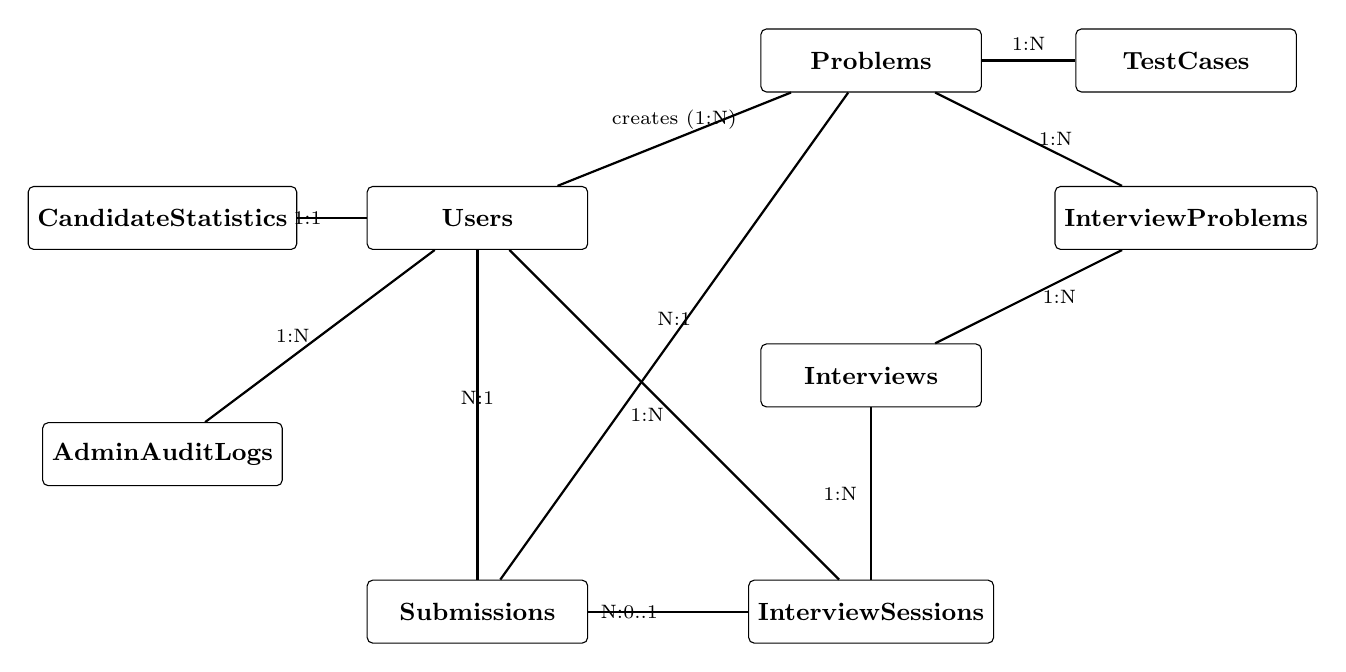
\begin{tikzpicture}[
    entity/.style={draw, rectangle, rounded corners=2pt,
                   minimum width=2.8cm, minimum height=0.8cm,
                   align=center, font=\small\bfseries},
    rel/.style={draw, thick},
    lbl/.style={font=\scriptsize, midway, above}
]

% Noduri (tabele)
\node[entity] (users)        at (0,0)       {Users};
\node[entity] (problems)     at (5,2)       {Problems};
\node[entity] (testcases)    at (9,2)       {TestCases};
\node[entity] (interviews)   at (5,-2)      {Interviews};
\node[entity] (iproblems)    at (9,0)       {InterviewProblems};
\node[entity] (isessions)    at (5,-5)      {InterviewSessions};
\node[entity] (submissions)  at (0,-5)      {Submissions};
\node[entity] (candstat)     at (-4,0)      {CandidateStatistics};
\node[entity] (auditlogs)    at (-4,-3)     {AdminAuditLogs};

% Users → Problems (1:N, CreatedByUserId)
\draw[rel] (users) -- node[lbl]{crea\-tes (1:N)} (problems);

% Users → CandidateStatistics (1:1)
\draw[rel] (users) -- node[lbl,left]{1:1} (candstat);

% Users → AdminAuditLogs (1:N)
\draw[rel] (users) -- node[lbl,left]{1:N} (auditlogs);

% Problems → TestCases (1:N)
\draw[rel] (problems) -- node[lbl]{1:N} (testcases);

% Interviews → InterviewProblems (1:N)
\draw[rel] (interviews) -- node[lbl,right]{\,1:N} (iproblems);

% Problems → InterviewProblems (1:N)
\draw[rel] (problems) -- node[lbl,right]{1:N} (iproblems);

% Interviews → InterviewSessions (1:N)
\draw[rel] (interviews) -- node[lbl,left]{1:N\,} (isessions);

% Users → InterviewSessions (1:N, CandidateId)
\draw[rel] (users) -- node[lbl,left]{1:N} (isessions);

% Submissions → Users (N:1)
\draw[rel] (submissions) -- node[lbl,above]{N:1} (users);

% Submissions → Problems (N:1)
\draw[rel] (submissions) -- node[lbl]{N:1} (problems);

% Submissions → InterviewSessions (N:1, nullable)
\draw[rel] (submissions) -- node[lbl,left]{N:0..1} (isessions);

\end{tikzpicture}
\caption{Diagrama entitate-relație a bazei de date.
  Relațiile reflectă cheile externe din
  \texttt{AppDbContextModelSnapshot.cs}.}
\label{fig:erd}
\end{figure}

% ─────────────────────────────────────────────────────────────────────────

\subsection{Secvența pipeline-ului de feedback AI}
\label{subsec:diagrama_secventa_ai}

Figura~\ref{fig:seq_ai} prezintă fluxul asincron complet de la trimiterea
submisiei până la afișarea feedback-ului în interfața candidatului.

\begin{figure}[ht]
\centering
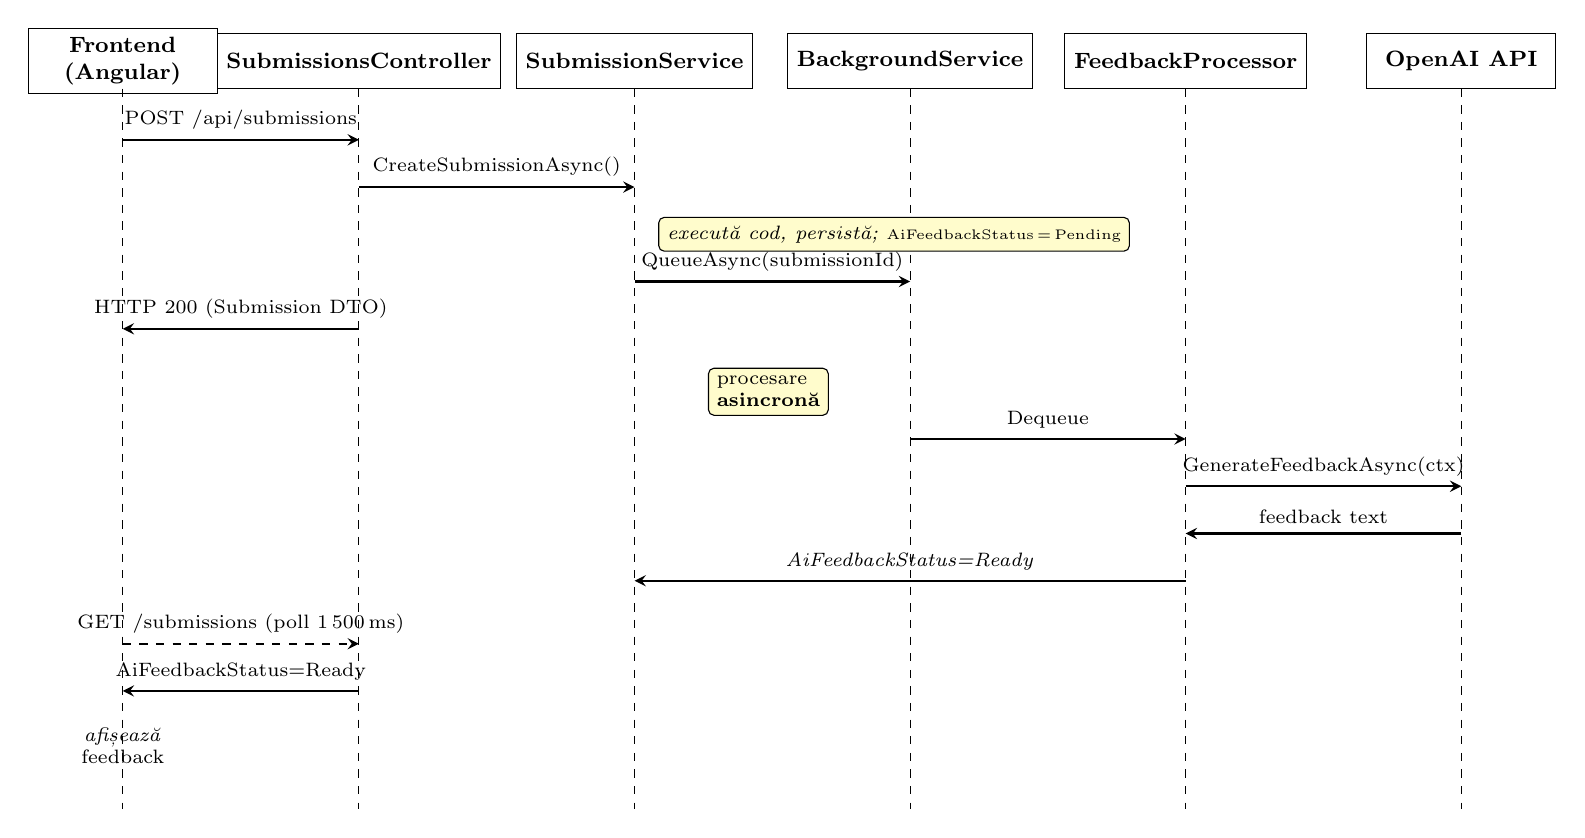
\begin{tikzpicture}[
    actor/.style={draw, rectangle, minimum width=2.4cm,
                  minimum height=0.7cm, align=center, font=\footnotesize\bfseries},
    lifeline/.style={draw, dashed, thin},
    msg/.style={->, thick, >=stealth, font=\scriptsize},
    asyncmsg/.style={->, thick, dashed, >=stealth, font=\scriptsize},
    note/.style={draw, rectangle, rounded corners=2pt, fill=yellow!20,
                 font=\scriptsize, align=left, inner sep=3pt}
]

% Actori
\node[actor] (fe)       at (0,0)    {Frontend\\(Angular)};
\node[actor] (ctrl)     at (3,0)    {SubmissionsController};
\node[actor] (svc)      at (6.5,0)  {SubmissionService};
\node[actor] (bg)       at (10,0)   {BackgroundService};
\node[actor] (proc)     at (13.5,0) {FeedbackProcessor};
\node[actor] (ai)       at (17,0)   {OpenAI API};

% Linii de viață
\foreach \x in {0, 3, 6.5, 10, 13.5, 17} {
    \draw[lifeline] (\x,-0.35) -- (\x,-9.5);
}

% 1. POST /api/submissions
\draw[msg] (0,-1) -- node[above]{POST /api/submissions} (3,-1);
% 2. CreateSubmissionAsync
\draw[msg] (3,-1.6) -- node[above]{CreateSubmissionAsync()} (6.5,-1.6);
% 3. ExecCode + Persist (notă internă pe lifeline-ul SubmissionService)
\node[note, anchor=west] at (6.8,-2.2)
    {\textit{execută cod, persistă;} {\tiny AiFeedbackStatus\,=\,Pending}};
% 4. QueueAsync
\draw[msg] (6.5,-2.8) -- node[above]{QueueAsync(submissionId)} (10,-2.8);
% 5. HTTP 200
\draw[msg] (3,-3.4) -- node[above]{HTTP 200 (Submission DTO)} (0,-3.4);

% --- asincron ---
\node[note] at (8.2,-4.2) {procesare\\\textbf{asincronă}};

% 6. Dequeue
\draw[msg] (10,-4.8) -- node[above]{Dequeue} (13.5,-4.8);
% 7. ProcessAsync
\draw[msg] (13.5,-5.4) -- node[above]{GenerateFeedbackAsync(ctx)} (17,-5.4);
% 8. OpenAI response
\draw[msg] (17,-6.0) -- node[above]{feedback text} (13.5,-6.0);
% 9. Save Ready
\draw[msg] (13.5,-6.6) -- node[above]{\textit{AiFeedbackStatus=Ready}} (6.5,-6.6);

% 10. Polling
\draw[asyncmsg] (0,-7.4) -- node[above]{GET /submissions (poll 1\,500\,ms)} (3,-7.4);
% 11. Return
\draw[msg] (3,-8.0) -- node[above]{AiFeedbackStatus=Ready} (0,-8.0);
% 12. Afișare
\node[font=\scriptsize, align=center] at (0,-8.7)
    {\textit{afișează}\\feedback};

\end{tikzpicture}
\caption{Diagrama de secvență a pipeline-ului de feedback AI.
  Generarea feedback-ului este complet asincronă față de cererea HTTP.}
\label{fig:seq_ai}
\end{figure}

% ─────────────────────────────────────────────────────────────────────────

\subsection{Diagrama cazurilor de utilizare}
\label{subsec:diagrama_use_case}

Figura~\ref{fig:use_case} ilustrează acțiunile disponibile pentru fiecare
dintre cele trei roluri: \textbf{Candidate}, \textbf{Interviewer} și
\textbf{Admin}.

\begin{figure}[ht]
\centering
\begin{tikzpicture}[
    actor/.style={font=\small\bfseries},
    uc/.style={draw, ellipse, minimum width=3.5cm, minimum height=0.7cm,
               align=center, font=\scriptsize},
    sys/.style={draw, rectangle, dashed, rounded corners=4pt,
                inner sep=12pt, font=\small\itshape},
    uses/.style={->, thin, >=stealth}
]

% Sistem
\node[sys, minimum width=11cm, minimum height=13cm] (system) at (5.5,-5.5) {};
\node[font=\small\itshape] at (5.5,-11.8) {AI Interview Coach};

% Cazuri de utilizare
\node[uc] (register)    at (5.5, -0.5) {Înregistrare / Autentificare};
\node[uc] (viewproblem) at (5.5, -1.8) {Vizualizare problemă};
\node[uc] (submit)      at (5.5, -3.0) {Trimitere soluție (C\#/Py/C++)};
\node[uc] (hint)        at (5.5, -4.2) {Solicită hint AI};
\node[uc] (feedback)    at (5.5, -5.4) {Vizualizare feedback AI};
\node[uc] (startint)    at (5.5, -6.6) {Accesare interviu (token)};
\node[uc] (createint)   at (5.5, -7.8) {Creare/gestionare interviuri};
\node[uc] (watchsess)   at (5.5, -9.0) {Monitorizare sesiuni candidați};
\node[uc] (adminproblem)at (5.5,-10.2) {Administrare probleme și catalog};
\node[uc] (auditlog)    at (5.5,-11.4) {Consultare audit și observabilitate};

% Actori
\node[actor] (candidate)   at (-2.5, -3.0)  {Candidate};
\node[actor] (interviewer) at (-2.5, -8.0)  {Interviewer};
\node[actor] (admin)       at (13.5, -5.5)  {Admin};

% Candidate → use cases
\foreach \uc in {register, viewproblem, submit, hint, feedback, startint} {
    \draw[uses] (candidate) -- (\uc);
}

% Interviewer → use cases
\foreach \uc in {register, viewproblem, createint, watchsess} {
    \draw[uses] (interviewer) -- (\uc);
}

% Admin → use cases (linii drepte din dreapta)
\foreach \uc in {register, viewproblem, submit, hint, feedback, startint, createint, watchsess, adminproblem, auditlog} {
    \draw[uses] (admin) -- (\uc);
}

\end{tikzpicture}
\caption{Diagrama cazurilor de utilizare pentru rolurile Candidate,
  Interviewer și Admin.
  Admin moștenește toate cazurile de utilizare ale celorlalte roluri.}
\label{fig:use_case}
\end{figure}
